\documentclass[11pt,a4paper]{article}

\usepackage{Act}

\begin{document}
\input{\detokenize{/home/fenarius/Travail/Cours/cpge-info/latex/Macros.tex}}
\ModeExercice
\TD{18}{Modèle entité-association}
\newcommand{\SPATH}{/home/fenarius/Travail/Cours/cpge-info/docs/mp2i/files/C18/}


\psset{treesep=0.5cm,levelsep=0.8cm}

\setcounter{Exercise}{0}

\begin{Exercise}[title = {Matériel informatique}, origin = {\bac \; Oraux {\sc ccinp}}]\\
    On considère le schéma de base de données suivant, qui décrit un ensemble de fabricants de matériel informatique, les matériels qu'ils vendent, leurs clients et ce qu'achètent leurs clients. Les attributs des clés primaires des six premières relations sont soulignés.
    \begin{itemize}
        \item {\tt Production(\underline{NomFabricant}, \underline{Modele})}
        \item {\tt Ordinateur(\underline{Modele}, Frequence, Ram, Dd, Prix)}
        \item {\tt Portable(\underline{Modele}, Frequence, Ram, Dd, Ecran, Prix)}
        \item {\tt Imprimante(\underline{Modele}, Couleur, Type, Prix)}
        \item {\tt Fabricant(\underline{Nom}, Adresse, NomPatron)}
        \item {\tt Client(\underline{Num}, Nom, Prenom)}
        \item {\tt Achat(NumClient, NomFabricant, Modele, Quantite)}
    \end{itemize}
Chaque client possède un numéro unique connu de tous les fabricants. La relation {\tt Production} donne pour chaque fabricant l'ensemble des modèles fabriquées par ce fabricant. Deux fabricants différents peuvent proposer le même matériel. La relation {\tt Ordinateur} donne pour chaque modèle d'ordinateur la vitesse du processeur (en Hz), les tailles de la Ram et du disque dur (en GO) et le prix de l'ordinateur (en \euro{}). La relation {\tt Portable}, en plus des attributs précédents, comporte la taille de l'écran (en pouces). La relation {\tt Imprimante} indique pour chaque modèle d'imprimante si elle imprime en couleur (vrai/faux), le type d'impression (laser ou jet d'encre) et le prix (en \euro{}). La relation {\tt Fabricant} stocke les noms et adresses de chaque fabricant, ainsi que le nom de son patron. La relation {\tt Client} stocke les noms et prénoms de tous les clients de tous les fabricants. Enfin, la relation {\tt Achat} regroupe les quadruplets (client $c$, fabricant $f$, modèle $m$ et quantité $q$) tel que le client de numéro $c$ a acheté $q$ fois le modèle $m$ au fabricant de nom $f$. On suppose que l'attribut {\tt Quantite} est toujours strictement positif.
\Question{Proposer une clé primaire pour la relation {\tt Achat}, quelles sont les conséquences en terme de modélisation ?}
\Question{Identifier l'ensemble des clés étrangères éventuelles de chaque table.}
\Question{Donner en {\sc sql} des requêtes répondant aux questions suivantes :}
\subQuestion{Quels sont les numéros de modèles des matériels (ordinateur, portable ou imprimante) fabriqués par  l’entreprise de nom Durand ?}
\subQuestion{Quels sont les noms et adresses des fabricants produisant des portables dont le disque dur a une capacité d’au moins 500 Go ?}
\subQuestion{Quels sont les noms des fabricants qui produisent au moins 10 modèles différents d’imprimantes ?}
\subQuestion{Quels sont les numéros des clients n’ayant acheté aucune imprimante ?}

\end{Exercise}

\begin{Exercise}[title={Cinémas}, origin={\bac \; {\sc ccinp} sujet zéro}]\\
    On considère la base de données décrite par le modèle entité-association suivant :
    \begin{center}
        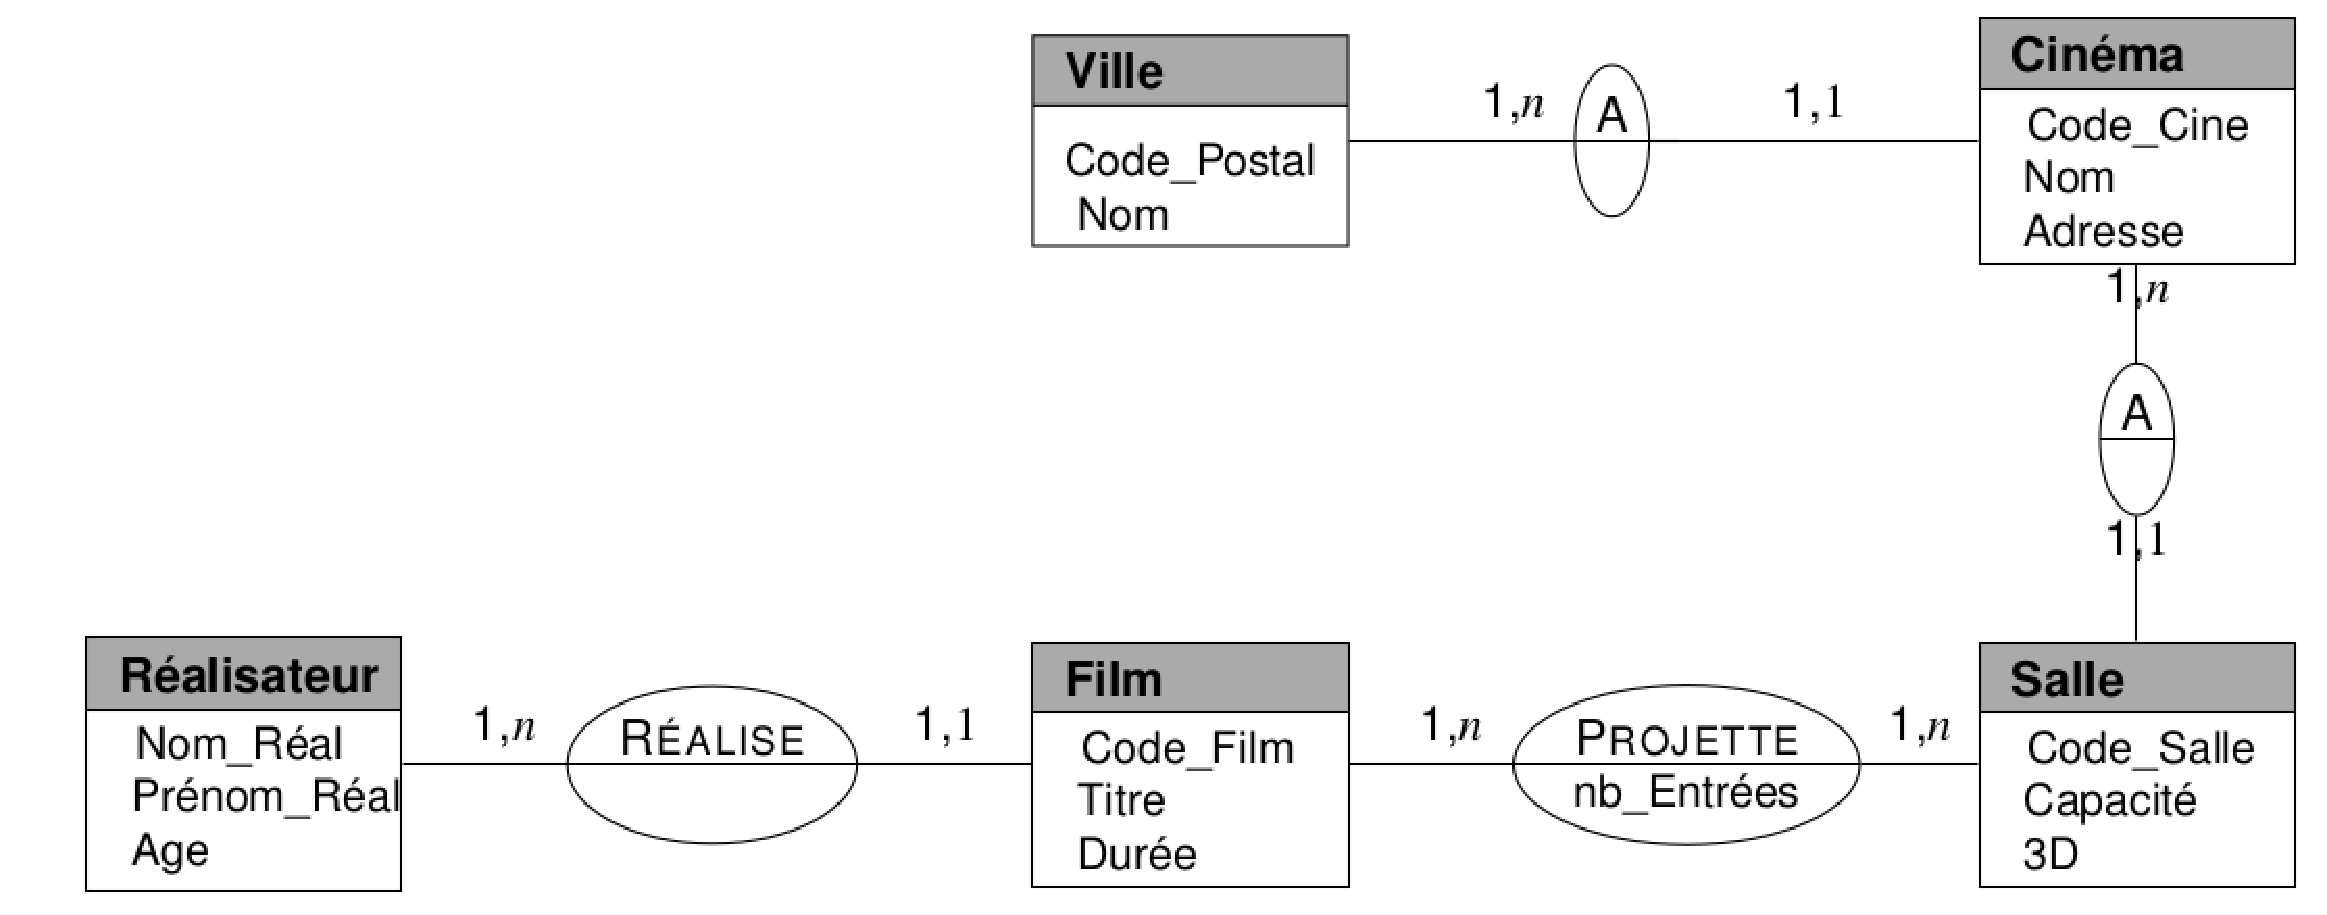
\includegraphics[width=400px]{ea1.eps}
    \end{center}
    Dans cette représentation, on lie des entités par des associations avec des cardinalités. Ainsi par exemple 
    \begin{center}
        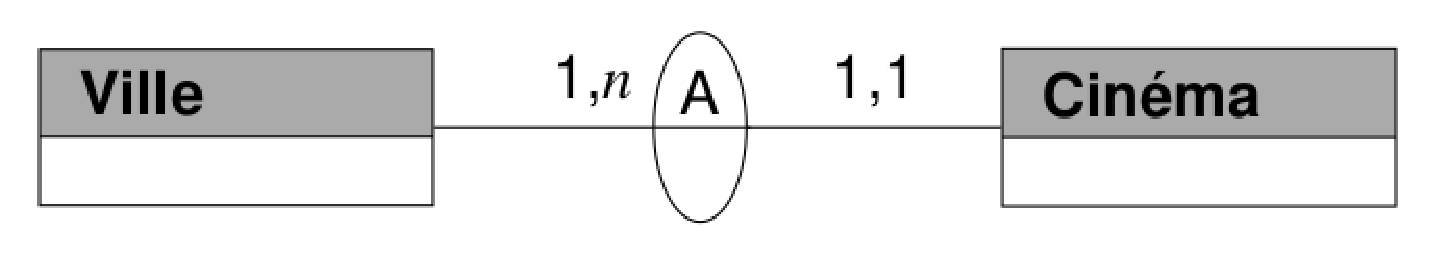
\includegraphics[height=40px]{ea2.eps}
    \end{center}
    peut se lire comme \og{} \textit{Une ville a 1 à n cinéma(s)} \fg{} et \og{} \textit{un cinéma est présent dans une et une seule ville} \fg{}. Parfois, l'association possède des propriétés (le nombre d'entrées d'un film projeté dans une salle par exemple).
    \smallskip
    On suppose que le champ {\sc 3d} de l'entité Salle est un entier, valant 0 si la salle n'est pas en {\sc 3d} et 1 sinon. On suppose de plus que la durée des films est en heures. Enfin, on affirme qu'une ville peut-être uniquement déterminé par son code postal et son nom.
    \Question{Donner le schéma relationnel correspondant. Préciser les clés primaires et étrangères des relations. Les clés primaires peuvent être associées à plusieurs attributs.}
    \Question{Ecrire les requêtes suivantes en langage {\sc sql} :}
    \subQuestion{Donner le titre des films durant moins de 2h.}
    \subQuestion{Donner le nom et le prénom du réalisateur ayant réalisé le film \og{} Matrix \fg{}.}
    \subQuestion{Compter le nombre de cinémas à Nantes.}
    \subQuestion{Donner l'adresse des cinémas contenant au moins une salle {\sc 3d}.}
    \subQuestion{Donner le code des films projetés dans toutes les salles.}
    \subQuestion{Donner la liste des titres des films projetés dans le cinéma \og{} Le Rio \fg{}.}

\end{Exercise}


\end{document}